\documentclass[11pt,preprint]{elsarticle}

\usepackage{lmodern}
%%%% My spacing
\usepackage{setspace}
\setstretch{1.2}
\DeclareMathSizes{12}{14}{10}{10}

% Wrap around which gives all figures included the [H] command, or places it "here". This can be tedious to code in Rmarkdown.
\usepackage{float}
\let\origfigure\figure
\let\endorigfigure\endfigure
\renewenvironment{figure}[1][2] {
    \expandafter\origfigure\expandafter[H]
} {
    \endorigfigure
}

\let\origtable\table
\let\endorigtable\endtable
\renewenvironment{table}[1][2] {
    \expandafter\origtable\expandafter[H]
} {
    \endorigtable
}


\usepackage{ifxetex,ifluatex}
\usepackage{fixltx2e} % provides \textsubscript
\ifnum 0\ifxetex 1\fi\ifluatex 1\fi=0 % if pdftex
  \usepackage[T1]{fontenc}
  \usepackage[utf8]{inputenc}
\else % if luatex or xelatex
  \ifxetex
    \usepackage{mathspec}
    \usepackage{xltxtra,xunicode}
  \else
    \usepackage{fontspec}
  \fi
  \defaultfontfeatures{Mapping=tex-text,Scale=MatchLowercase}
  \newcommand{\euro}{€}
\fi

\usepackage{amssymb, amsmath, amsthm, amsfonts}

\def\bibsection{\section*{References}} %%% Make "References" appear before bibliography


\usepackage[numbers]{natbib}

\usepackage{longtable}
\usepackage[margin=2.3cm,bottom=2cm,top=2.5cm, includefoot]{geometry}
\usepackage{fancyhdr}
\usepackage[bottom, hang, flushmargin]{footmisc}
\usepackage{graphicx}
\numberwithin{equation}{section}
\numberwithin{figure}{section}
\numberwithin{table}{section}
\setlength{\parindent}{0cm}
\setlength{\parskip}{1.3ex plus 0.5ex minus 0.3ex}
\usepackage{textcomp}
\renewcommand{\headrulewidth}{0pt}

\usepackage{array}
\newcolumntype{x}[1]{>{\centering\arraybackslash\hspace{0pt}}p{#1}}

%%%%  Remove the "preprint submitted to" part. Don't worry about this either, it just looks better without it:
\journal{Journal of Finance}

 \def\tightlist{} % This allows for subbullets!

\usepackage{hyperref}
\hypersetup{breaklinks=true,
            bookmarks=true,
            colorlinks=true,
            citecolor=blue,
            urlcolor=blue,
            linkcolor=blue,
            pdfborder={0 0 0}}


% The following packages allow huxtable to work:
\usepackage{siunitx}
\usepackage{multirow}
\usepackage{hhline}
\usepackage{calc}
\usepackage{tabularx}
\usepackage{booktabs}
\usepackage{caption}


\newenvironment{columns}[1][]{}{}

\newenvironment{column}[1]{\begin{minipage}{#1}\ignorespaces}{%
\end{minipage}
\ifhmode\unskip\fi
\aftergroup\useignorespacesandallpars}

\def\useignorespacesandallpars#1\ignorespaces\fi{%
#1\fi\ignorespacesandallpars}

\makeatletter
\def\ignorespacesandallpars{%
  \@ifnextchar\par
    {\expandafter\ignorespacesandallpars\@gobble}%
    {}%
}
\makeatother


% definitions for citeproc citations
\NewDocumentCommand\citeproctext{}{}
\NewDocumentCommand\citeproc{mm}{%
\href{\#cite.\detokenize{#1}}{#2}\nocite{#1}}

\makeatletter
% allow citations to break across lines
\let\@cite@ofmt\@firstofone
% avoid brackets around text for \cite:
\def\@biblabel#1{}
\def\@cite#1#2{{#1\if@tempswa , #2\fi}}
\makeatother
\newlength{\cslhangindent}
\setlength{\cslhangindent}{1.5em}
\newlength{\csllabelwidth}
\setlength{\csllabelwidth}{3em}
\newenvironment{CSLReferences}[2] % #1 hanging-indent, #2 entry-spacing
{\begin{list}{}{%
	\setlength{\itemindent}{0pt}
	\setlength{\leftmargin}{0pt}
	\setlength{\parsep}{0pt}
	% turn on hanging indent if param 1 is 1
	\ifodd #1
	\setlength{\leftmargin}{\cslhangindent}
	\setlength{\itemindent}{-1\cslhangindent}
	\fi
	% set entry spacing
	\setlength{\itemsep}{#2\baselineskip}}}
{\end{list}}

\usepackage{calc}
\newcommand{\CSLBlock}[1]{\hfill\break\parbox[t]{\linewidth}{\strut\ignorespaces#1\strut}}
\newcommand{\CSLLeftMargin}[1]{\parbox[t]{\csllabelwidth}{\strut#1\strut}}
\newcommand{\CSLRightInline}[1]{\parbox[t]{\linewidth - \csllabelwidth}{\strut#1\strut}}
\newcommand{\CSLIndent}[1]{\hspace{\cslhangindent}#1}


\urlstyle{same}  % don't use monospace font for urls
\setlength{\parindent}{0pt}
\setlength{\parskip}{6pt plus 2pt minus 1pt}
\setlength{\emergencystretch}{3em}  % prevent overfull lines
\setcounter{secnumdepth}{5}

%%% Use protect on footnotes to avoid problems with footnotes in titles
\let\rmarkdownfootnote\footnote%
\def\footnote{\protect\rmarkdownfootnote}
\IfFileExists{upquote.sty}{\usepackage{upquote}}{}

%%% Include extra packages specified by user
\usepackage{booktabs}
\usepackage{longtable}
\usepackage{array}
\usepackage{multirow}
\usepackage{wrapfig}
\usepackage{float}
\usepackage{colortbl}
\usepackage{pdflscape}
\usepackage{tabu}
\usepackage{threeparttable}
\usepackage{threeparttablex}
\usepackage[normalem]{ulem}
\usepackage{makecell}
\usepackage{xcolor}

%%% Hard setting column skips for reports - this ensures greater consistency and control over the length settings in the document.
%% page layout
%% paragraphs
\setlength{\baselineskip}{12pt plus 0pt minus 0pt}
\setlength{\parskip}{12pt plus 0pt minus 0pt}
\setlength{\parindent}{0pt plus 0pt minus 0pt}
%% floats
\setlength{\floatsep}{12pt plus 0 pt minus 0pt}
\setlength{\textfloatsep}{20pt plus 0pt minus 0pt}
\setlength{\intextsep}{14pt plus 0pt minus 0pt}
\setlength{\dbltextfloatsep}{20pt plus 0pt minus 0pt}
\setlength{\dblfloatsep}{14pt plus 0pt minus 0pt}
%% maths
\setlength{\abovedisplayskip}{12pt plus 0pt minus 0pt}
\setlength{\belowdisplayskip}{12pt plus 0pt minus 0pt}
%% lists
\setlength{\topsep}{10pt plus 0pt minus 0pt}
\setlength{\partopsep}{3pt plus 0pt minus 0pt}
\setlength{\itemsep}{5pt plus 0pt minus 0pt}
\setlength{\labelsep}{8mm plus 0mm minus 0mm}
\setlength{\parsep}{\the\parskip}
\setlength{\listparindent}{\the\parindent}
%% verbatim
\setlength{\fboxsep}{5pt plus 0pt minus 0pt}



\begin{document}



\begin{frontmatter}  %

\title{Loans and Credit}

% Set to FALSE if wanting to remove title (for submission)




\author[Add1]{Anya Nash}
\ead{25051911@sun.ac.za}





\address[Add1]{Stellenbosch University, Stellenbosch, South Africa}

\cortext[cor]{Corresponding author: Anya Nash}


\vspace{1cm}





\vspace{0.5cm}

\end{frontmatter}

\setcounter{footnote}{0}



%________________________
% Header and Footers
%%%%%%%%%%%%%%%%%%%%%%%%%%%%%%%%%
\pagestyle{fancy}
\chead{}
\rhead{}
\lfoot{}
\rfoot{}
\lhead{}
%\rfoot{\footnotesize Page \thepage } % "e.g. Page 2"
\cfoot{}

%\setlength\headheight{30pt}
%%%%%%%%%%%%%%%%%%%%%%%%%%%%%%%%%
%________________________

\headsep 35pt % So that header does not go over title




\subsection{Default Profile Summary
Statistics}\label{default-profile-summary-statistics}

\subsubsection{Default Rate by Grade}\label{default-rate-by-grade}

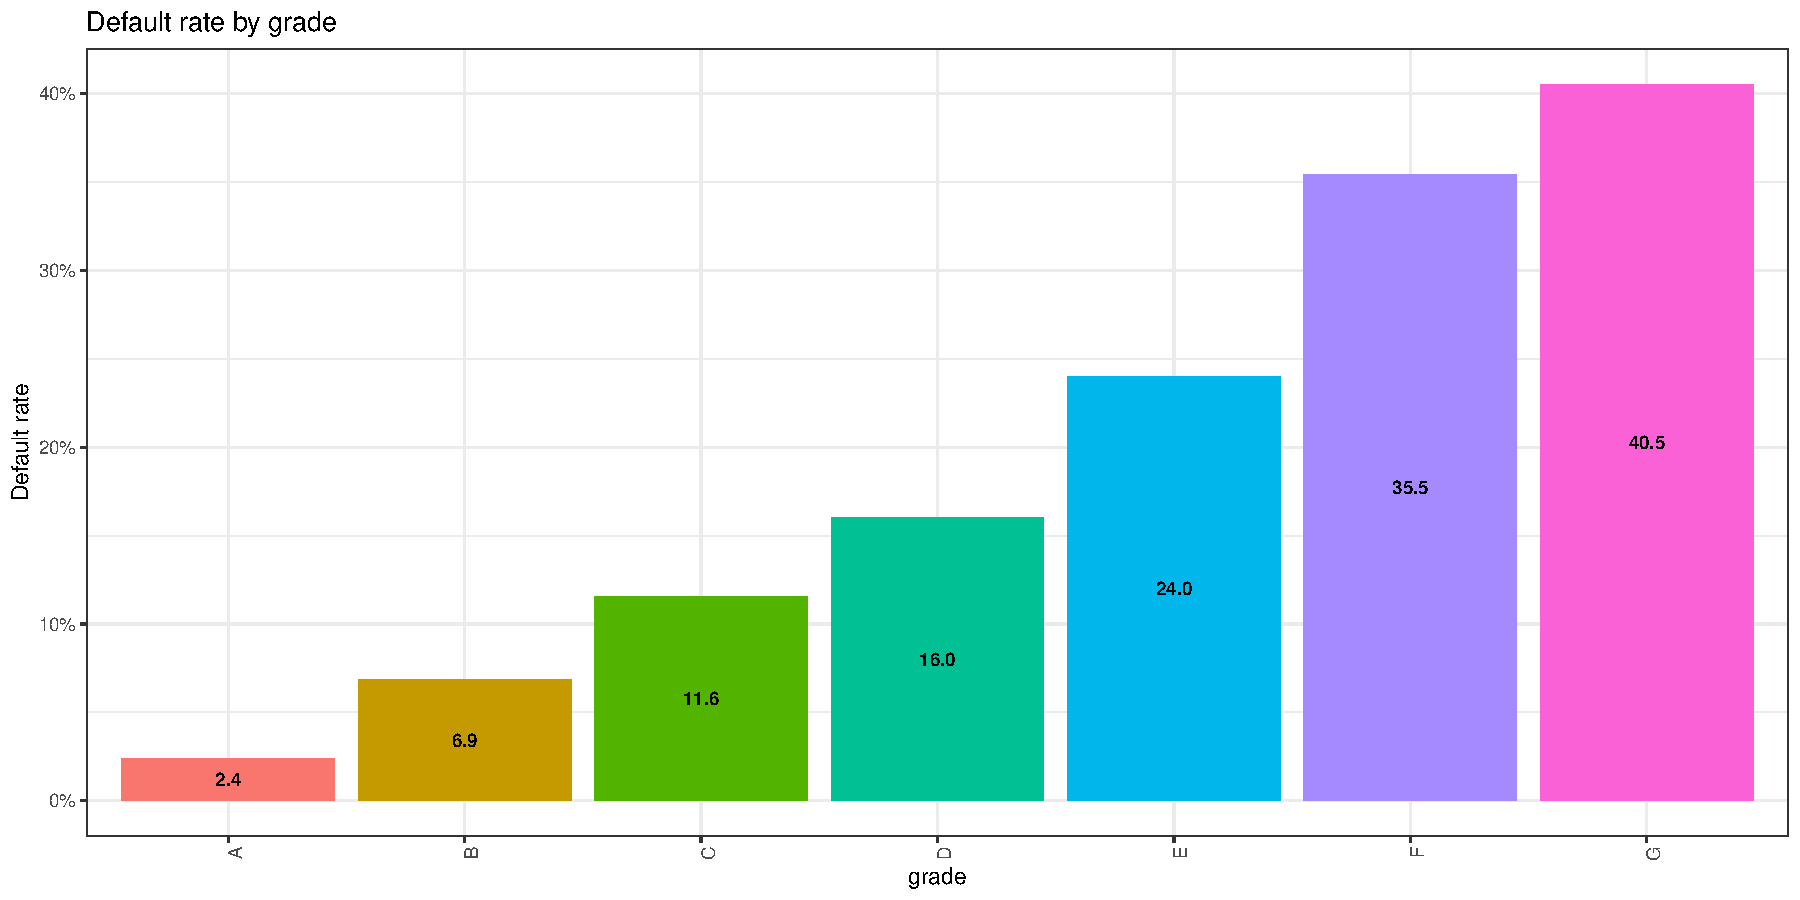
\includegraphics[width=1\linewidth]{25051911_Question_3_files/figure-latex/unnamed-chunk-3-1}

It is clear from the graph that as credit grade goes from A to G, the
default rate increases exponentially. Therefore, grade is highly
associated with the default rate (although that is how it is designed).

\subsubsection{Default Rate by Term of
Loan}\label{default-rate-by-term-of-loan}


\includegraphics[width=1\linewidth]{25051911_Question_3_files/figure-latex/unnamed-chunk-4-1}

There is a small difference in the default rate based on the length of
the loan, with the longer loan having a slightly higher default rate.

\subsubsection{Default Rate by Length of
Employment}\label{default-rate-by-length-of-employment}


\includegraphics[width=1\linewidth]{25051911_Question_3_files/figure-latex/unnamed-chunk-5-1}

There is not a substantial difference in the default rate based on the
length of employment, except for those who have n/a for length of
employment - they have a much higher default rate. This is logical,
because those who answered n/a to length of employment are most likely
not working/ unemployed. Thus, they probably have a less stable income,
which would make their default rate higher.

\subsubsection{Default Rate by State}\label{default-rate-by-state}

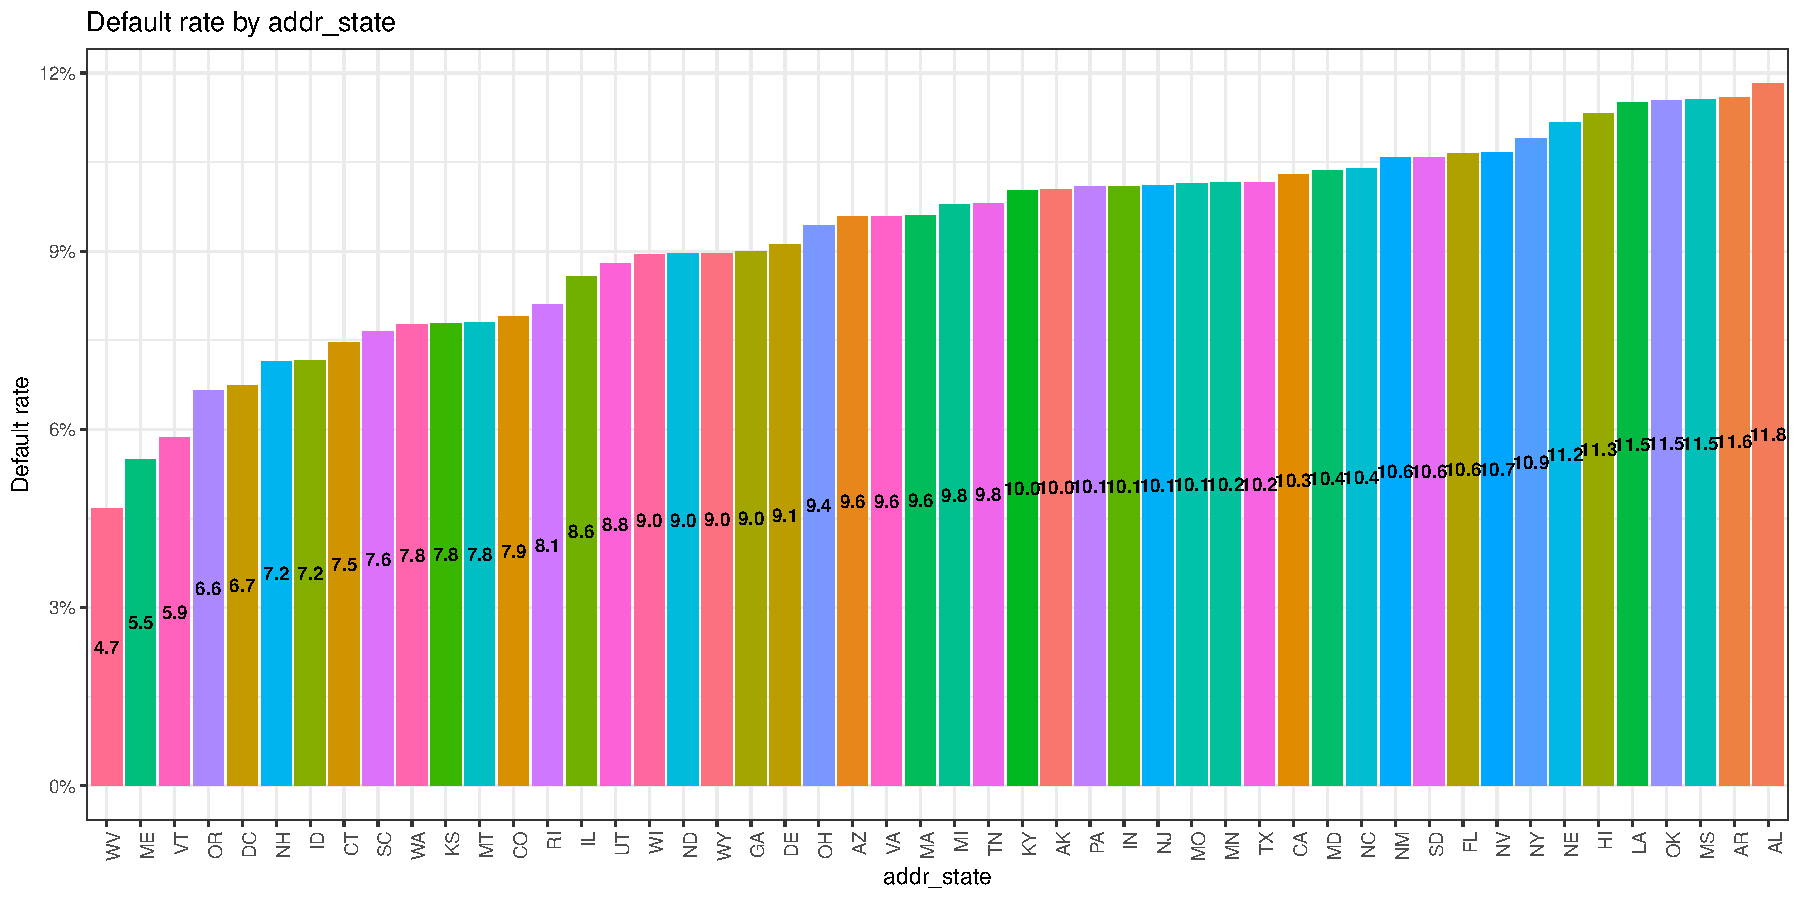
\includegraphics[width=1\linewidth]{25051911_Question_3_files/figure-latex/unnamed-chunk-6-1}

There is no obvious outlier in the default rate based on US state,
however, the difference in default rate between the state with the
highest default rate (Alabama) and the state with the lowest default
rate (West Virginia) is substantial. Texas has a default rate on the
higher side, however, it is not obviously different from any of the
other states.

\subsubsection{Default Rate by State for Short Term
Loans}\label{default-rate-by-state-for-short-term-loans}


\includegraphics[width=1\linewidth]{25051911_Question_3_files/figure-latex/unnamed-chunk-7-1}

There is no obvious outlier in the default rate based on US state for
short term loans, however, the difference in default rate between the
state with the highest default rate (Alabama) and the state with the
lowest default rate (West Virginia) is substantial. Texas has a default
rate on the higher side, however, it is not obviously different from any
of the other states.

\subsubsection{Default Rate by DTI Band}\label{default-rate-by-dti-band}


\includegraphics[width=1\linewidth]{25051911_Question_3_files/figure-latex/unnamed-chunk-8-1}

The default rate for different bands of the debt-to-income ratio follows
an expected pattern. The default rate is lower for a lower
debt-to-income ratio, and the default rate is higher for a higher
debt-to-income ratio.

\subsubsection{Default Rate by Purpose of
Loan}\label{default-rate-by-purpose-of-loan}

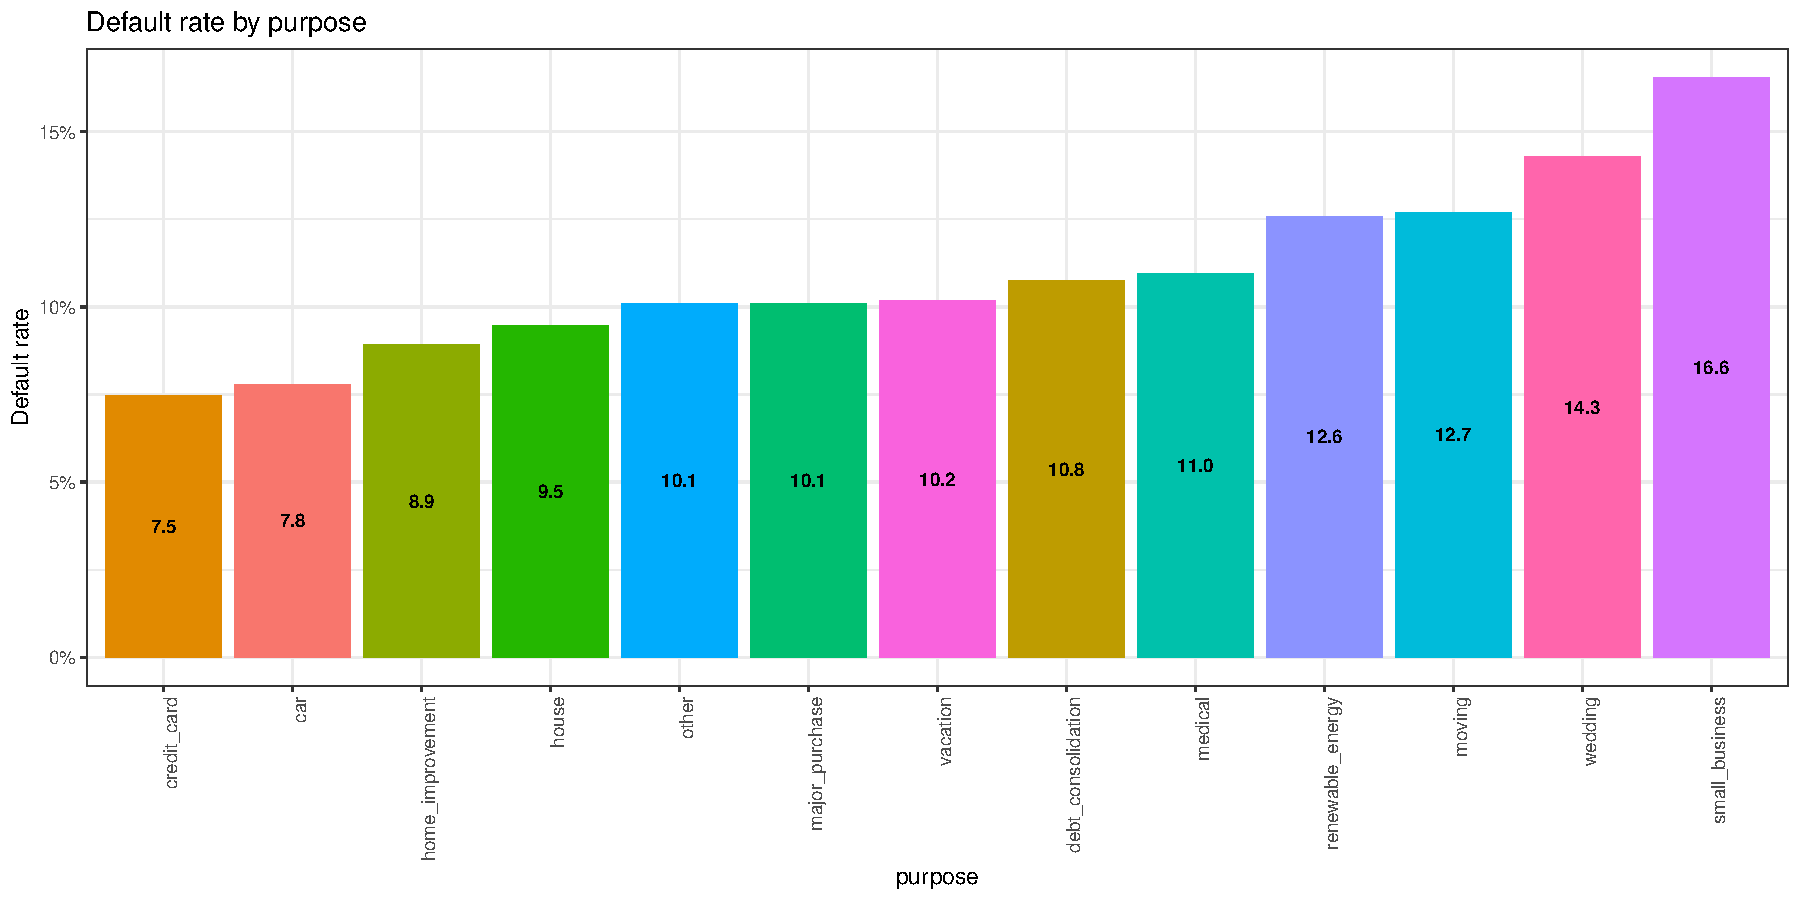
\includegraphics[width=1\linewidth]{25051911_Question_3_files/figure-latex/unnamed-chunk-9-1}

The default rate differs a bit based on the purpose of the loan. Loans
for paying off credit cards or buying cars have the lowest default rate,
while loans for weddings and small businesses have the highest default
rate. It is logical that loans for small businesses have the highest
default rate, since small businesses often carry a higher investment
risk, and have unpredictable profits (and often low/ no initial
profits).

\subsection{Default Rate, Credit Grades and Young
Individuals}\label{default-rate-credit-grades-and-young-individuals}

Unfortunately, there is no age variable in the data. Therefore, as a
very rough, imperfect proxy for age, I use length of employment. I
classify young individuals as those with a length of employment of 5
years or less. Then, to determine whether credit grades are a good
indicator for whether younger individuals will default on their loans, I
regress the default rate on credit grade, restricting the sample to
younger individuals only. The table below shows the results of the
regression.

\begin{longtable}[t]{lrrrr}
\caption{\label{tab:unnamed-chunk-11}Regression of default rate on loan grade}\\
\toprule
Variable & Estimate & Std. Error & t-statistic & p-value\\
\midrule
Constant & 0.024 & 0.001 & 24.097 & 0\\
Grade B & 0.048 & 0.001 & 36.969 & 0\\
Grade C & 0.097 & 0.001 & 74.878 & 0\\
Grade D & 0.141 & 0.002 & 90.907 & 0\\
Grade E & 0.221 & 0.002 & 98.887 & 0\\
\addlinespace
Grade F & 0.331 & 0.004 & 84.018 & 0\\
Grade G & 0.391 & 0.008 & 51.708 & 0\\
\bottomrule
\end{longtable}

As seen in the regression table above, credit grade is a somewhat good
indicator of whether younger individuals will default. This is because
all the coefficients are statistically significant with an
economically-meaningful magnitude, however, the R-squared value is quite
low at 0.04928, meaning there are many other factors that influence the
default rate of young individuals.

\subsection{Interest Rates, Age, Occupation and Credit
Scores}\label{interest-rates-age-occupation-and-credit-scores}

Using employment length as an imperfect, rough proxy for age once again
and using very rough occupation categories, I regress interest rate on
employment length, occupation and credit score to determine whether
interest rates are determined by these factors. The results are
displayed below.

\begin{verbatim}
## OLS estimation, Dep. Var.: int_rate
## Observations: 786,940
## Fixed-effects: grade: 7,  emp_length: 12,  emp_title_clean: 43,388
## RMSE: 1.3155   Adj. R2: 0.926009
\end{verbatim}

With an R-squared value of 0.926009, it is clear that interest rates are
strongly associated with age, occupation and credit scores.

\subsection{Risk Profiles}\label{risk-profiles}

The table below shows the top 10 combinations of credit grade, DTI band,
purpose of loan and type of home ownership that have the highest default
rates.

\begin{longtable}[]{@{}
  >{\centering\arraybackslash}p{(\linewidth - 12\tabcolsep) * \real{0.0636}}
  >{\centering\arraybackslash}p{(\linewidth - 12\tabcolsep) * \real{0.0909}}
  >{\centering\arraybackslash}p{(\linewidth - 12\tabcolsep) * \real{0.1818}}
  >{\centering\arraybackslash}p{(\linewidth - 12\tabcolsep) * \real{0.1455}}
  >{\centering\arraybackslash}p{(\linewidth - 12\tabcolsep) * \real{0.1909}}
  >{\centering\arraybackslash}p{(\linewidth - 12\tabcolsep) * \real{0.1273}}
  >{\centering\arraybackslash}p{(\linewidth - 12\tabcolsep) * \real{0.2000}}@{}}
\caption{Top 10 borrower profiles with the highest default
rates}\tabularnewline
\toprule\noalign{}
\begin{minipage}[b]{\linewidth}\centering
Grade
\end{minipage} & \begin{minipage}[b]{\linewidth}\centering
DTI band
\end{minipage} & \begin{minipage}[b]{\linewidth}\centering
Loan purpose
\end{minipage} & \begin{minipage}[b]{\linewidth}\centering
Home ownership
\end{minipage} & \begin{minipage}[b]{\linewidth}\centering
Number of borrowers
\end{minipage} & \begin{minipage}[b]{\linewidth}\centering
Default rate
\end{minipage} & \begin{minipage}[b]{\linewidth}\centering
Median annual income
\end{minipage} \\
\midrule\noalign{}
\endfirsthead
\toprule\noalign{}
\begin{minipage}[b]{\linewidth}\centering
Grade
\end{minipage} & \begin{minipage}[b]{\linewidth}\centering
DTI band
\end{minipage} & \begin{minipage}[b]{\linewidth}\centering
Loan purpose
\end{minipage} & \begin{minipage}[b]{\linewidth}\centering
Home ownership
\end{minipage} & \begin{minipage}[b]{\linewidth}\centering
Number of borrowers
\end{minipage} & \begin{minipage}[b]{\linewidth}\centering
Default rate
\end{minipage} & \begin{minipage}[b]{\linewidth}\centering
Median annual income
\end{minipage} \\
\midrule\noalign{}
\endhead
\bottomrule\noalign{}
\endlastfoot
G & (30,35{]} & debt\_consolidation & RENT & 202 & 53.5\% & \$55,500 \\
G & (25,30{]} & debt\_consolidation & RENT & 159 & 46.5\% & \$56,000 \\
F & (30,35{]} & debt\_consolidation & RENT & 597 & 44.7\% & \$50,119 \\
F & (20,25{]} & debt\_consolidation & RENT & 716 & 43.7\% & \$60,000 \\
G & (30,35{]} & debt\_consolidation & MORTGAGE & 186 & 41.9\% &
\$65,000 \\
F & (25,30{]} & debt\_consolidation & RENT & 685 & 41.8\% & \$55,000 \\
G & (20,25{]} & debt\_consolidation & RENT & 172 & 40.7\% & \$57,450 \\
F & (35,40{]} & debt\_consolidation & RENT & 295 & 40.0\% & \$50,000 \\
G & (15,20{]} & debt\_consolidation & RENT & 118 & 39.8\% & \$55,674 \\
F & (15,20{]} & debt\_consolidation & RENT & 628 & 39.5\% & \$62,000 \\
\end{longtable}

From the table above, we can see that the highest defaulters are
individuals with credit grades of either F or G, a DTI that is greater
than 25 and who rent their homes. The median income for each group is
between 50000 and 60000 US dollars.

When lenders assess borrower credibility, they can do a number of things
to reduce default risk. They can identify those borrowers who are part
of the highest default risk combination categories and either reduce the
loan amount to these borrowers, or have additional checks and balances
before approving the loan. Instead of just focusing on one category or
``tick-box'' at a time, lenders now have a better, fuller picture of the
default risk of the borrower. A borderline answer for one or two
categories could be viewed as okay when each category is viewed in
isolation, but could paint a much riskier picture when categories are
viewed together.

\subsection{DTI Cap}\label{dti-cap}

The table below shows how the share of loans accepted and default rate
would change, if there was a DTI cap imposed.

\begin{longtable}[t]{cccc}
\caption{\label{tab:unnamed-chunk-16}Default risk under alternative DTI hard caps}\\
\toprule
DTI cap & Borrowers accepted & Share accepted & Default rate\\
\midrule
5 & 47688 & 5.3\% & 7.7\%\\
10 & 164287 & 18.1\% & 7.6\%\\
15 & 341407 & 37.7\% & 8.0\%\\
20 & 528833 & 58.4\% & 8.5\%\\
25 & 684950 & 75.6\% & 9.0\%\\
\addlinespace
30 & 798324 & 88.1\% & 9.4\%\\
35 & 864625 & 95.4\% & 9.8\%\\
40 & 891675 & 98.4\% & 9.9\%\\
45 & 896435 & 98.9\% & 9.9\%\\
50 & 899763 & 99.3\% & 9.9\%\\
\addlinespace
55 & 901461 & 99.5\% & 9.9\%\\
\bottomrule
\end{longtable}

As seen in the table above, as the DTI cap increases, both the share
accepted and default rate increase. Therefore, there is a trade-off
between the risk of default and maximising the number of borrowers. A
DTI cap that is too strict will cause the number of borrowers to decline
significantly, however, it would also have the positive effect of
reducing the default rate. The same goes for a DTI cap that is too
lenient - the number of borrowers will increase, but at the cost of the
default rate increasing as well. I think an appropriate hard-cap for DTI
levels is 25. At 25, approximately 75\% of borrowers are accepted, which
is not too low, and the default rate is at 9\%, which is an improvement
compared to no DTI cap.

\bibliography{Tex/ref}





\end{document}
